%%%%%%%%%%%%%%%%%%%%%%%%%%%%%%%%%%%%%%%%%%%%%%%%%%%%%%%%%%%%%%%%%%%%%%%%%%%%%%%%%%%%%%%
% 	FYP Report - Lee Wei Yeong (lwy08)	%
%%%%%%%%%%%%%%%%%%%%%%%%%%%%%%%%%%%%%%%%%%%%%%%%%%%%%%%%%%%%%%%%%%%%%%%%%%%%%%%%%%%%%%%
\documentclass{icldt}
\def \supervisor   {Prof. Susan Eisenbach}
\def \secondmarker {Dr. Tristan Allwood}
%%%%%%%%%%%%%%%%%%%%%%%%%%%%%%%%%%%%%%%%%%%%%%%%%%%%%%%%%%%%%%%%%%%%%%%%%%%%%%%%%%%%%%%
\usepackage{amsmath, amssymb, amsthm} % AMS packages
\usepackage{graphicx}                 % Packages for graphics and color
\usepackage[usenames,dvipsnames]{color}
\usepackage[T1]{fontenc}              % Ensure correct text encoding
\usepackage[utf8]{inputenc}
\usepackage{url}
\usepackage{algorithm, algorithmic}
\usepackage{subfigure}
\usepackage{moreverb}
\usepackage{eukdate}
\usepackage[british]{babel}
\usepackage{parskip}				% justified paragraphs + newlines
\usepackage{minted}
\usepackage{appendix}
\usepackage{xcolor}
\usepackage{fancyvrb}
\usepackage{courier, listings}
\usepackage{tocbasic}
\usepackage{proof}
\usepackage{mathrsfs}
\usepackage{enumerate}
\usepackage{float,multicol,epsfig}
\usepackage{turnstile}
\usepackage{mathtools,extarrows}
\usepackage{tikz}					% figure drawing library
\usetikzlibrary{calendar,calc,trees,positioning,arrows,chains,shapes.geometric,%
    decorations.pathreplacing,decorations.pathmorphing,shapes,%
    matrix,shapes.symbols}
\usepackage{tikz-qtree}
\usepackage{verbatim}
\lstset{basicstyle=\footnotesize\ttfamily,breaklines=true}
\usepackage{mathpazo}				% custom fonts

% manage vertical spacing
\usepackage{etex}
\usepackage[compact]{titlesec}
\titleformat{\chapter}[display]
  {\normalfont\huge\bfseries}{\chaptertitlename\ \thechapter}{20pt}{\Huge}
\titlespacing*{\chapter}{0pt}{-22pt}{11pt}
\titlespacing*{\section}{0pt}{11pt}{0pt}
\titlespacing*{\subsection}{0pt}{11pt}{0pt}
\titlespacing*{\subsubsection}{0pt}{5pt}{0pt}

% custom captions
\usepackage[hang, small, bf, margin=0pt]{caption}
\DeclareCaptionFont{white}{\color{white}}
\DeclareCaptionFormat{listing}{\colorbox{gray}{\parbox{\textwidth}{#1#2#3}}}
\captionsetup[lstlisting]{format=listing,labelfont=white,textfont=white}
\setlength{\abovecaptionskip}{0pt}

% PDF options
\usepackage[pdftex,bookmarks=true,colorlinks]{hyperref}
\usepackage[figure,table]{hypcap} % Correct a problem with hyperref
\hypersetup{
    bookmarksnumbered,
    pdfstartview={FitH},
    citecolor={black},
    linkcolor={black},
    urlcolor={black},
    pdfpagemode={UseOutlines},
    pdfborder={0 0 0}
}
% hack to ensure the hyperlinks actually jump to the right place
\makeatletter
\newcommand\org@hypertarget{}
\let\org@hypertarget\hypertarget
\renewcommand\hypertarget[2]{%
\Hy@raisedlink{\org@hypertarget{#1}{}}#2%
} \makeatother

% page layout
\parindent 0pt
\setlength{\parsep}{0pt}
\setlength{\topskip}{0pt}
\setlength{\topmargin}{0pt}
\setlength{\topsep}{0pt}
\setlength{\partopsep}{0pt}
\setlength{\footskip}{30pt}
\numberwithin{equation}{section}       % Tinker with equation numbering
\renewcommand{\bibname}{References}    % Alter appearance of table of contents slightly
\renewcommand{\contentsname}{Contents}
\pagenumbering{arabic}

% fix for \float@addtolists warning
\usepackage{scrhack}
\usepackage{fancyhdr}
\setlength{\headheight}{14pt}
\pagestyle{fancy}
\renewcommand{\headrulewidth}{0pt}
\renewcommand{\footrulewidth}{0pt}
\fancyhf{} % clear all header and footer fields
\fancyhead[RH]{\slshape \leftmark}
\fancyfoot[C]{\thepage}

% extension for simple column horizontal stretching
\usepackage{tabularx}

% insert chapter reference by name
\usepackage{nameref}

% enable multi-line text node support
\usepackage{makecell}

% for project timetable
\usepackage{colortbl}
\definecolor{lgray}{gray}{0.8}

\lstdefinelanguage{CSharp}
{
 morecomment = [l]{//}, 
 morecomment = [l]{///},
 morecomment = [s]{/*}{*/},
 morestring=[b]", 
 sensitive = true,
 morekeywords = {abstract,  event,  new,  struct,
   as,  explicit,  null,  switch,
   base,  extern,  object,  this,
   bool,  false,  operator,  throw,
   break,  finally,  out,  true,
   byte,  fixed,  override,  try,
   case,  float,  params,  typeof,
   catch,  for,  private,  uint,
   char,  foreach,  protected,  ulong,
   checked,  goto,  public,  unchecked,
   class,  if,  readonly,  unsafe,
   const,  implicit,  ref,  ushort,
   continue,  in,  return,  using,
   decimal,  int,  sbyte,  virtual,
   default,  interface,  sealed,  volatile,
   delegate,  internal,  short,  void,
   do,  is,  sizeof,  while,
   double,  lock,  stackalloc,   
   else,  long,  static,   
   enum,  namespace,  string}
}

\def\naive{na\"{\i}ve }

% tikz settings for architecture diagram
\tikzset{
>=stealth',
  value/.style={
    text width=10em, 
    minimum height=3em, 
    text centered, 
    on chain},
  component/.style={
    rectangle, 
    rounded corners,
    draw=black, very thick,
    text width=10em, 
    minimum height=3em, 
    text centered, 
    on chain},
  line/.style={draw, thick, <-},
  element/.style={
    tape,
    top color=white,
    bottom color=blue!50!black!60!,
    minimum width=8em,
    draw=blue!40!black!90, very thick,
    text width=10em, 
    minimum height=3.5em, 
    text centered, 
    on chain},
  every join/.style={->, thick,shorten >=1pt},
  decoration={brace},
  category/.style={decorate},
  catlabel/.style={midway, right=2pt},
}

%%%%%%%%%%%%%%%%%%%%%%%%%%%%%%%%%%%%%%%%%%%%%%%%%%%%%%%%%%%%%%%%%%%%%%%%%%%%%%%%%%%%%%%
\begin{document}
	%Font Sizes
%\tiny
%\scriptsize
%\footnotesize
%\small
%\normalsize
%\large
%\Large
%\LARGE
%\huge
%\Huge

\begin{titlepage}
\begin{center}
\textsc{\Large Imperial College London\\Department of Computing}
\vfil
{\Huge{\textbf{Pyrulan}}}\linebreak \linebreak
{\huge Automated lazy testing for Python}
\vfil
{\LARGE Final Year Individual Project}\linebreak \linebreak
{\LARGE Interim Report (draft)}\\[2cm]
{\Large Lee Wei Yeong }
\vfil
{\Large Supervisor: \supervisor} \linebreak \linebreak
{\Large Second Marker: \secondmarker}
\vfil
{\Large \monthname\ \number\year}
\end{center}
\end{titlepage}

%%%%%%%%%%%%%%%%%%%%%%%%%%%%%%%%%%%%%%%%%%%%%%%%%%%%%%%%%%%%%%%%%%%%%%%%%%%%%%%%%%%%%%%
\begin{abstract}
Lorem ipsum dolor sit amet, consectetur adipiscing elit. In risus. Ut vitae velit. Aenean malesuada adipiscing sem. Quisque ligula mauris, posuere sed, elementum id, suscipit et, urna. Phasellus suscipit tristique nisl. Vivamus ac urna. Pellentesque egestas facilisis velit. Class aptent taciti sociosqu ad litora torquent per conubia nostra, per inceptos himenaeos. Morbi eu augue. Vestibulum congue placerat sem. Integer eget urna id risus suscipit eleifend. Etiam at est. Class aptent taciti sociosqu ad litora torquent per conubia nostra, per inceptos himenaeos. Praesent orci. Suspendisse potenti. Morbi egestas, justo vel cursus eleifend, dui leo dapibus ante, vitae pretium purus massa sed enim. Vivamus eu libero in nulla sagittis aliquam. Quisque semper quam id dui. Nulla facilisi.	
%	\hfill --- Pyrulan
\end{abstract}
%%%%%%%%%%%%%%%%%%%%%%%%%%%%%%%%%%%%%%%%%%%%%%%%%%%%%%%%%%%%%%%%%%%%%%%%%%%%%%%%%%%%%%%
	\chapter*{Acknowledgements}

First of all, I would like to thank Professor Susan Eisenbach for supervising my project, and giving me invaluable advice and guidance throughout my work.

Secondly, I thank Dr. Tristan Allwood for his support, ideas, encouragement, and the useful discussions that we had regarding the direction of my project.

Also, many thanks to Chong-U Lim for his insight during our conversations, as well as to Yangfan Zhang, a close friend, without whom this project would not be what it is.

Finally, I would like to thank my family for their continued full support during the course of my university studies.

%%%%%%%%%%%%%%%%%%%%%%%%%%%%%%%%%%%%%%%%%%%%%%%%%%%%%%%%%%%%%%%%%%%%%%%%%%%%%%%%%%%%%%%
	\tableofcontents
%\listoftables
%\listoffigures
%%%%%%%%%%%%%%%%%%%%%%%%%%%%%%%%%%%%%%%%%%%%%%%%%%%%%%%%%%%%%%%%%%%%%%%%%%%%%%%%%%%%%%%
\chapter{Introduction}
\begin{comment}
\begin{itemize}
	\item What is the problem?
	\item Why is it interesting / important / difficult to solve / issues to address?
	\item What is your main idea for solving it?
\end{itemize}
\end{comment}
%%%%%%%%%%%%%%%%%%%%%%%%%%%%%%%%%%%%%%%%%%%%%%%%%%%%%%%%%%%%%%%%%%%%%%%%%%%%%%%%%%%%%%%
\section{Motivation}	% describes the continual need for automated testing
Professional software engineers often write tests while developing code, especially for large complex codebases. These tests are highly beneficial for generating confidence in a bug-free solution delivery.

However, writing tests is not easy to get right, and can be quite costly. It is reported that testing code is responsible for approximately half the total cost of software development \cite{Edvardsson99asurvey}\cite{Han2008}\cite{Korel2005}.

Furthermore, this task becomes gradually more time-consuming as software grows in terms of complexity. Given similar resource constraints, it can become increasingly difficult to consistently achieve high test code coverage.

Moreover, a significant proportion of overall development time is spent writing test code, which is eventually not included in production. Hence this work, though critical to software quality assurance \cite{Harrold00}, is ultimately hidden from the client, as far as billing and accountability is concerned.

This has led to a large body of work on automatically generating test suites in the imperative programming community \cite{Allwood2011}.

Even then, the present need for manual testing indicates that there still remains much scope for improvement in this area. A recent example supporting this claim is Google handing out a record \$26k in bug bounties for security researchers reporting Chrome vulnerabilities \cite{ChromeBugBounties}.

Therefore, this raises the question of whether full automatic discovery \cite{Bertolino2007} for all these bugs could be possible, in order to eliminate this cost, let alone any bug exploits.
%%%%%%%%%%%%%%%%%%%%%%%%%%%%%%%%%%%%%%%%%%%%%%%%%%%%%%%%%%%%%%%%%%%%%%%%%%%%%%%%%%%%%%%
\section{Automated software testing for dynamic languages}
Whilst research in this field is typically devoted to static programming languages such as Java or C/C++, relatively less emphasis is placed on their dynamic counterparts like Javascript, Ruby or Python.

One such paper implements search-based software testing (SBST) technique, to automatically generate test scenarios for Ruby code, using genetic algorithms \cite{Mairhofer2011}. There is no equivalent tool targeting Python instead.

This observation is made in contrast to the rapid growth trend in popularity of dynamic languages, especially in recent years, and in particular, Python. Python was awarded the TIOBE Programming Language of the Year in 2007 and 2010 \cite{TiobeDec11}.

In this paper \cite{Mairhofer2011}, the authors claimed success in achieving consistent and significantly high code coverage over a preselected set of test inputs with their tool, when compared against the \naive random test case generator. Would it be possible to better this using a suitable adaptation of existing techniques, and/or to maintain this coverage across a more extensive range of programs?

As both Python and Ruby are reflective and dynamic languages, it would be logical to adopt a similar approach in solving this problem, specifically by generating test scenarios via \emph{runtime code analysis} \cite{Mairhofer2011}.
%%%%%%%%%%%%%%%%%%%%%%%%%%%%%%%%%%%%%%%%%%%%%%%%%%%%%%%%%%%%%%%%%%%%%%%%%%%%%%%%%%%%%%%
\section{Python}
The Python programming language contains a variety of interesting features which encourage rapid experimentation with automatic testing techniques.

This is primarily because Python is an open source, general purpose, multi-paradigm, cross-platform compatible, dynamically typed language, offering duck typing, and in active development and support. It also provides \emph{excellent builtin introspection and reflection capabilities}, to inspect and manipulate code at runtime.

At the heart of the language design philosophy \cite{Pep20ZenPython}, there should be one-- and preferably only one --obvious way to do it. The importance of readability promotes a \emph{clean, concise and elegant syntax}, advantageous to easily demonstrate proof of concepts.

For instance, the Python code snippet reads more fluently than its C\# counterpart:

\begin{tabularx}{\textwidth}{X X}
\underline{Sample C\# code} & \underline{Equivalent Python code} \\
\begin{lstlisting}[language=CSharp]^^J
if ("hello".indexOf("e") >= 0)^^J
\{^^J
\ \ \ return true;^^J
\}^^J
\end{lstlisting}
&
\begin{lstlisting}[language=python]^^J
if 'e' in 'hello':^^J
\ \ \ return True^^J
\end{lstlisting}
\end{tabularx}
Apart from the fundamental testing infrastructure toolset of \textsf{unittest}, \textsf{doctest} and \textsf{py.test} offered in Python, there is limited availability of testing support tools built on top of this. Many of these either target outdated versions of Python, or are discontinued. There are even fewer of such tools for automated testing, for instance, \textsf{pythoscope} and \textsf{pytestsgenerator}, which generate tests by performing static code analysis, and a lack of any automated dynamic test case generators at all.
%%%%%%%%%%%%%%%%%%%%%%%%%%%%%%%%%%%%%%%%%%%%%%%%%%%%%%%%%%%%%%%%%%%%%%%%%%%%%%%%%%%%%%%
\section{Project contributions}
Within the context given above, this project makes the following key contributions:

\begin{itemize}
	\item A discussion of the possible ways considered for automated software testing, focusing on test data generation by only using information gathered at runtime
	\item A motivating example describing automated lazy testing in Python
	\item Implementation as a Python module to automatically generate high coverage test suites, primarily evaluated against Python libraries like Django web framework, NumPy/SciPy, wxPython
	\item Investigating effectiveness of the lazy testing technique, as illustrated by \textsc{Irulan} in Haskell \cite{Allwood2011}, for Python
	\item Further advance the work in the field of automated software testing, especially for dynamic languages
\end{itemize}

To this end, we take advantage of the main features of the Python language, ie. strong introspection and reflective capabilities, together with its extensive tool support, the Python Package Index (PyPI) repository.

The concepts discussed in this paper are concretely demonstrated in a tool called \textsc{Pyrulan}, a high coverage test suite generator for Python library code, written in Python. This tool has successfully been applied to some of the most popular frameworks, and achieved the initial objective of consistently high test code coverage, discovering several bugs in the process as well. The tool has also been extended to conducted property and regression testing, where reports on a sample of case studies are included.

\section{Report organisation}
The rest of this paper is structured as follows. Firstly, relevant background material is reviewed in Chapter \ref{ch:background}. Thereafter, the various algorithms and techniques used to automatically generate tests are formally introduced in Chapter \ref{ch:research}. These ideas presented here are then implemented in the tool \textsc{Pyrulan}, constituting the subject of Chapter \ref{ch:pyrulan}. This is accompanied by a detailed description of its software design architecture, together with several worked examples for clarification. Summarising, the success of the project is discussed in Chapter \ref{ch:eval}, before some final conclusions are drawn and suggestions are given to possible future work in Chapter \ref{ch:conclusion}.
%%%%%%%%%%%%%%%%%%%%%%%%%%%%%%%%%%%%%%%%%%%%%%%%%%%%%%%%%%%%%%%%%%%%%%%%%%%%%%%%%%%%%%%
\chapter{Background}
\label{ch:background}
\section{Introduction}
This part of the paper is intended to provide an overview and discussion of the relevant literature to this project, forming the basis for the reader to follow later content. Firstly, Sections \ref{sect:basics} to \ref{sect:overview} review the general field of automated software testing. Section \ref{sect:current-state} deals with the papers that inspired and influenced this project. Relevant characteristics of dynamically typed programming languages, with special focus on Python, are then discussed in Section \ref{sect:python-features}. Finally, the associated technical difficulties are highlighted in Section \ref{sect:challenges}.
%%%%%%%%%%%%%%%%%%%%%%%%%%%%%%%%%%%%%%%%%%%%%%%%%%%%%%%%%%%%%%%%%%%%%%%%%%%%%%%%%%%%%%%
\section{Basic concepts}
\label{sect:basics}
Software testing delivers quality assurance in the product to the customer. It verifies that software bugs are absent, as far as verification that implementation complies with original client specification goes. The following terms commonly found in \emph{automated test data generation research} are defined below.

\subsection{Definition of terms}
\subsubsection{General testing}
\begin{itemize}
	\item \emph{Test data}: data specifically identified for use in testing the software
	\item \emph{Test case}: set of conditions under which the correct behaviour of an application is determined
	\item \emph{Test suite}: a collection of test cases
	\item \emph{Test automation}: use of software to control test execution, comparison of actual and expected results, setting up of test preconditions, and other test control and reporting functions
	\item \emph{Test coverage}: measurement of extent to which software has been exercised by tests
\end{itemize}

\subsubsection{Graph theory}
\begin{itemize}
	\item \emph{Path}: sequence of nodes and edges. If a path begins from the entry node, and terminates at the exit node, then it is a \emph{complete} path.
	\item \emph{Branch predicate}: condition in a node leading to either a true or false path
	\item \emph{Path predicate}: collection of branch predicates which are required to be true, in order to traverse the path
	\item \emph{Feasible path}: path with valid input for execution
	\item \emph{Infeasible path}: path with no valid input for execution
	\item \emph{Constraint}: an expression of conditions imposed on variables to satisfy
\end{itemize}
%%%%%%%%%%%%%%%%%%%%%%%%%%%%%%%%%%%%%%%%%%%%%%%%%%%%%%%%%%%%%%%%%%%%%%%%%%%%%%%%%%%%%%%
\subsection{Validation criteria}
Software is usually checked for whether it meets certain functional, non-functional and business related requirements.

\subsubsection{Functional requirements}
Functional requirements are associated with specific product features and functionality.

\subsubsection{Non-functional requirements}
Non-functional requirements refer to product quality, in terms of constraints placed on attributes like speed, efficiency, reliability, safety and scalability. This is an area where automation excels in, over manual testing, and thus also becomes the key focus of this paper.

\subsubsection{Business requirements}
Business requirements reflect customer concerns, with respect to fulfilling the demands of daily work processes.
%%%%%%%%%%%%%%%%%%%%%%%%%%%%%%%%%%%%%%%%%%%%%%%%%%%%%%%%%%%%%%%%%%%%%%%%%%%%%%%%%%%%%%%
\section{Implementations}
\subsection{Static method}
This method generate tests without executing the software, generally via symbolic execution to solve for constraints on input variables. The static approach to test case generation derives a test case that will traverse a chosen path, as it satisfies that path predicate.

This paper \cite{Tahbildar} mentions the problem of infeasible path detection in case of loops with a variable number of iterations, and claims that it is weaker than the dynamic method at gathering type information, hence it is useful only for straight forward code. The main difficulty in this technique is solving non-linear constraints.

\subsection{Dynamic method}
Instead of using variable substitution, software under test is executed (frequently more than one pass), with some selected input. Code instrumentation will monitor and report if program execution follows an intended path. Search methods can be varied to pursue more "interesting" paths. Variables are then updated each time before the next execution, until this goal is achieved, at which point, the associated test case is generated.

According to the paper \cite{Tahbildar}, the authors note that research has attempted to combine symbolic reasoning with dynamic execution, or modifying inputs by heuristic function minimisation techniques. However, problems such as scalability and non-termination of infeasible paths arise from this approach.

\subsection{Hybrid}
Recent research on test data generation combines both these methods to try to mitigate these disadvantages, in order to obtain high coverage of feasible execution paths. It does not traditionally enumerate through the entire program input space, but instead solves partial path predicates to generate test cases. Therefore, this paper intends to further explore this area, to improve the efficiency in automated test data generation.
%%%%%%%%%%%%%%%%%%%%%%%%%%%%%%%%%%%%%%%%%%%%%%%%%%%%%%%%%%%%%%%%%%%%%%%%%%%%%%%%%%%%%%%
\section{Overview}
\label{sect:overview}
The following diagram \cite{McMinn2004} outlines the different kinds of software testing:

\begin{tikzpicture}[
  	event/.style={text width=2cm,text centered,font=\sffamily,anchor=north},
  	edge from parent/.style={very thick,draw=black!64},
    	edge from parent path={(\tikzparentnode.south) -- ++(0,-0.5cm)
			-| (\tikzchildnode.north)},
	level 1/.style={sibling distance=4cm,level distance=1cm,
		growth parent anchor=south,nodes=event},
	level 2/.style={sibling distance=4cm},
	level 3/.style={sibling distance=4cm},
	level 4/.style={sibling distance=4cm}]

	\node {Software testing}
		child [yshift=1cm] {
			child {node [level 1] {Functional (blackbox)}
				child {node [level 2] {Specification}}
			}
			child {node [level 1] {Hybrid (greybox)}
				child {node [level 2,xshift=0.8cm] {Assertion}}
				child {node [level 2,xshift=-0.8cm] {Exception condition \cite{Tracey2002}}}
			}
			child {node [level 1,xshift=0.4cm] {Structural (whitebox)}
				child {node [level 2,xshift=0.8cm] {Static}
		     	      child {node [level 3] {Symbolic execution}}
				}
				child {node [level 2,xshift=0.4cm] {Dynamic}
	    	 	      child {node [level 3,text width=2.5cm,xshift=0.8cm,yshift=-0.4cm] {Systematic (optimisation)}
			      		child { node [level 4,xshift=0.8cm] {Genetic algorithm \cite{Mairhofer2011}}}
			      		child { node [level 4] {Simulated annealing}}
			      		child { node [level 4,xshift=-0.8cm] {Hill climbing}}
			      }
		     	      child {node [level 3,text width=2.5cm,xshift=-0.4cm] {Random\\ (with feedback)}}
				}
			}
		};
\end{tikzpicture}

Another interesting paper is the idea of testability transformations \cite{Korel2005}, where source code is refactored to facilitate software testing, like unrolling loops for example.
%%%%%%%%%%%%%%%%%%%%%%%%%%%%%%%%%%%%%%%%%%%%%%%%%%%%%%%%%%%%%%%%%%%%%%%%%%%%%%%%%%%%%%%
\section{Current state of the art}
\label{sect:current-state}
These reference survey papers \cite{McMinn2004} \cite{Han2008} \cite{Tahbildar} provide a high level overview of software testing techniques.

The closest automated unit test generator in a dynamic language is \textsc{RuTeG} \cite{Mairhofer2011}, which uses evolutionary algorithms on Ruby source code to automatically create unit tests in Ruby. Apart from the description in the paper, there is no source code available online to try it out.

With respect to automated test generation in Python, there is only minimal work done. The most recent tools, such as \href{http://pythoscope.org/tutorial}{\textsf{pythoscope}} v0.4.3 (Feb 2010) and \href{http://code.google.com/p/pytestsgenerator}{\textsf{pytestsgenerator}} v0.2 (Feb 2009), perform static analysis on Python source code, as opposed to dynamic testing on Python bytecode.

\subsection{Pythoscope}
Pythoscope is an open source unit test generator for Python code. It is able to create additional test cases for user-specified points of entry, and also appends new test cases, thus allowing the user to safely modify and extend generated test cases. An example usage is provided below to illustrate this application in action:

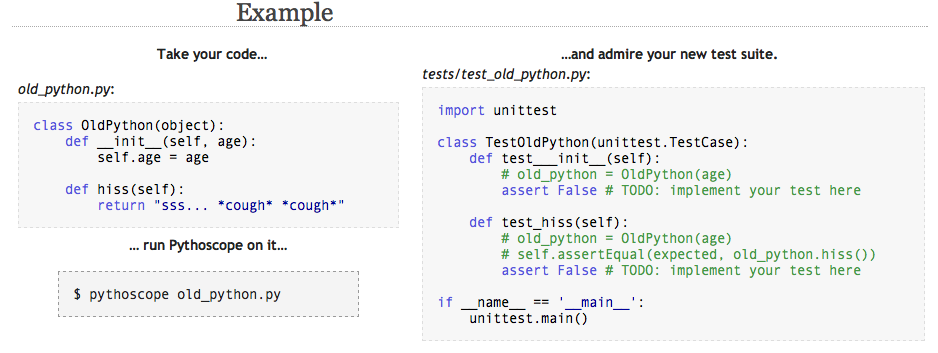
\includegraphics[scale=.46]{pythoscope.png}

\subsection{Python Tests Generator}
This automated test case generator creates unit tests for Python modules. The authors Vijakumar and Karthikeyan developed this tool on 32-bit Linux. Its purpose is to simplify usage of the existing PyUnit framework, and generate logical test cases for classes and methods. It also consists of a WxPython GUI, in addition to the CLI. The application is packaged for distribution using the \textsf{distutils} module.

According to accompanying documentation, this tool is intended to accomplish the following objectives:
\begin{itemize}
	\item Read a specified python module
	\item List the Classes, Functions and Properties of that module (for the user's selection)
	\item Drill down the Classes for methods and properties
	\item Generate basic set of test cases for each class or method selected
\end{itemize}

The predetermined logic for the test cases to be generated include:
\begin{itemize}
	\item Number of arguments
	\item Valid arguments
	\item Invalid arguments
	\item Custom logic
\end{itemize}

An example demonstration of the software follows:

\lstinputlisting[language=python,label=SourceCode,caption=Sample input Python program]{sample.py}

\lstinputlisting[language=python,label=GeneratedTests,caption=Generated unit test suite]{generated_tests.py}

\lstinputlisting[caption=Results of test execution]{output.txt}

\subsection{\textsc{Irulan}}
As for implementing the idea of lazy instantiation, \textsc{Irulan} \cite{Allwood2011} is the canonical tool written to demonstrate this concept in Haskell.

\textsc{Irulan} has four key objectives to achieve, which this project intends to do similarly, where possible:
\begin{enumerate}[1.]
	\item Automatic inference constructors and functions to generate test data
	\item Needed narrowing / lazy instantiation
	\item Inspection of elements inside returned data structures
	\item Efficiently handle polymorphism by (lazily) instantiating all possible instances
\end{enumerate}

A sample execution to discover errors in the following code snippet:
\definecolor{gray_ulisses}{gray}{0.55}
\definecolor{castanho_ulisses}{rgb}{0.71,0.33,0.14}
\definecolor{preto_ulisses}{rgb}{0.41,0.20,0.04}
\definecolor{green_ulises}{rgb}{0.2,0.75,0}
\lstdefinelanguage{HaskellUlisses} {
	basicstyle=\ttfamily\normalsize,
	sensitive=true,
	morecomment=[l][\color{gray_ulisses}\ttfamily\normalsize]{--},
	morecomment=[s][\color{gray_ulisses}\ttfamily\normalsize]{\{-}{-\}},
	morestring=[b]",
	stringstyle=\color{red},
	showstringspaces=false,
	numberstyle=\normalsize,
	numberblanklines=true,
	showspaces=false,
	breaklines=true,
	showtabs=false,
	emph=
	{[1]
		FilePath,IOError,abs,acos,acosh,all,and,any,appendFile,approxRational,asTypeOf,asin,
		asinh,atan,atan2,atanh,basicIORun,break,catch,ceiling,chr,compare,concat,concatMap,
		const,cos,cosh,curry,cycle,decodeFloat,denominator,digitToInt,div,divMod,drop,
		dropWhile,either,elem,encodeFloat,enumFrom,enumFromThen,enumFromThenTo,enumFromTo,
		error,even,exp,exponent,fail,filter,flip,floatDigits,floatRadix,floatRange,floor,
		fmap,foldl,foldl1,foldr,foldr1,fromDouble,fromEnum,fromInt,fromInteger,fromIntegral,
		fromRational,fst,gcd,getChar,getContents,getLine,head,id,inRange,index,init,intToDigit,
		interact,ioError,isAlpha,isAlphaNum,isAscii,isControl,isDenormalized,isDigit,isHexDigit,
		isIEEE,isInfinite,isLower,isNaN,isNegativeZero,isOctDigit,isPrint,isSpace,isUpper,iterate,
		last,lcm,length,lex,lexDigits,lexLitChar,lines,log,logBase,lookup,map,mapM,mapM_,max,
		maxBound,maximum,maybe,min,minBound,minimum,mod,negate,not,notElem,null,numerator,odd,
		or,ord,otherwise,pi,pred,primExitWith,print,product,properFraction,putChar,putStr,putStrLn,quot,
		quotRem,range,rangeSize,read,readDec,readFile,readFloat,readHex,readIO,readInt,readList,readLitChar,
		readLn,readOct,readParen,readSigned,reads,readsPrec,realToFrac,recip,rem,repeat,replicate,return,
		reverse,round,scaleFloat,scanl,scanl1,scanr,scanr1,seq,sequence,sequence_,show,showChar,showInt,
		showList,showLitChar,showParen,showSigned,showString,shows,showsPrec,significand,signum,sin,
		sinh,snd,span,splitAt,sqrt,subtract,succ,sum,tail,take,takeWhile,tan,tanh,threadToIOResult,toEnum,
		toInt,toInteger,toLower,toRational,toUpper,truncate,uncurry,undefined,unlines,until,unwords,unzip,
		unzip3,userError,words,writeFile,zip,zip3,zipWith,zipWith3,listArray,doParse
	},
	emphstyle={[1]\color{blue}},
	emph=
	{[2]
		Bool,Char,Double,Either,Float,IO,Integer,Int,Maybe,Ordering,Rational,Ratio,ReadS,ShowS,String,
		Word8,InPacket
	},
	emphstyle={[2]\color{castanho_ulisses}},
	emph=
	{[3]
		case,class,data,deriving,do,else,if,import,in,infixl,infixr,instance,let,
		module,of,primitive,then,type,where
	},
	emphstyle={[3]\color{preto_ulisses}\textbf},
	emph=
	{[4]
		quot,rem,div,mod,elem,notElem,seq
	},
	emphstyle={[4]\color{castanho_ulisses}\textbf},
	emph=
	{[5]
		EQ,False,GT,Just,LT,Left,Nothing,Right,True,Show,Eq,Ord,Num
	},
	emphstyle={[5]\color{preto_ulisses}\textbf}
}
\begin{lstlisting}[language=HaskellUlisses,frame=single]
module IntTreeExample where
data IntTree
	= Leaf
	| Branch IntTree Int IntTree
insert :: Int -> IntTree -> IntTree
insert n Leaf = Branch Leaf n Leaf
insert n (Branch left x right)
	| n < x = Branch (insert n left) x right
	| n > x = Branch left x (insert n right)
\end{lstlisting}

produces the following output:
\begin{lstlisting}[language=HaskellUlisses,frame=single]
$ irulan --ints='[0,1]' --enable-case-statements -a --maximumRuntime=1 source IntTreeExample
...
insert 1 (Branch ? 1 ?1) ==> !
IntTreeExample.hs:(8,0)-(11,41): Non-exhaustive patterns in function insert
insert 0 (Branch ? 0 ?1) ==> !
IntTreeExample.hs:(8,0)-(11,41): Non-exhaustive patterns in function insert
case insert 0 (Branch (Branch ? 0 ?1) 1 ?2) of
Branch x _ _ -> x ==> !
IntTreeExample.hs:(8,0)-(11,41): Non-exhaustive patterns in function insert
case case insert 0 (Branch (Branch (Branch ? 0 ?1) 1 ?2) 1 ?3) of
Branch x _ _ -> x of
Branch x _ _ -> x ==> !
IntTreeExample.hs:(8,0)-(11,41): Non-exhaustive patterns in function insert
...
\end{lstlisting}
%%%%%%%%%%%%%%%%%%%%%%%%%%%%%%%%%%%%%%%%%%%%%%%%%%%%%%%%%%%%%%%%%%%%%%%%%%%%%%%%%%%%%%%
\section{Features of Python}
\label{sect:python-features}
...
%%%%%%%%%%%%%%%%%%%%%%%%%%%%%%%%%%%%%%%%%%%%%%%%%%%%%%%%%%%%%%%%%%%%%%%%%%%%%%%%%%%%%%%
\section{Challenges}
\label{sect:challenges}
There are several facets of complexity to this problem, which this work hopes to tackle.
%%%%%%%%%%%%%%%%%%%%%%%%%%%%%%%%%%%%%%%%%%%%%%%%%%%%%%%%%%%%%%%%%%%%%%%%%%%%%%%%%%%%%%%
\subsection{Parameter instantiation}
Parameters refer to primitives, data structures like lists, maps or trees, and objects. Depending on available resources, scope might be restricted to only certain numeric types or specific functions, eg. methods invoking \texttt{strcmp()}.

This is especially applicable not only to class constructors when creating appropriate objects, but also automatically generating initial user input.

It is vital to ensure that an exhaustive search is not performed, because there would quickly be an exponential blow up, especially in functions with multiple input arguments, as well as being inefficient, due to many meaningless test cases.

There are several possible ways to conducting the search for such corner cases. Previous algorithms range from \naive systematic enumeration of all possible values to variants of random testing.

Therefore, the task here is to come up with a more efficient way of prioritising pathological boundary parameter value generation, under real time and space constraints. Some leading intuition follows.
%%%%%%%%%%%%%%%%%%%%%%%%%%%%%%%%%%%%%%%%%%%%%%%%%%%%%%%%%%%%%%%%%%%%%%%%%%%%%%%%%%%%%%%
\subsubsection{Lazy instantiation}
It might be reasonable to begin with ``lazy instantiation" \cite{Allwood2011}, where dummy nullified objects are passed in initially, and test data are only generated for return values when the methods on them are actually invoked. This supposes multiple runs through the same code block, and using feedback from previous iteration to direct future execution. A \href{https://github.com/evandrix/Pyrulan}{prototype} of this is available together with the original project proposal.

\subsubsection{Runtime in-memory manipulation}
It is also envisioned that the dynamic language features of Python be exploited in order to rapidly generate useful test data. One idea is to manipulate and observe the behaviour of code blocks in memory at runtime, by monkeypatching or hotswapping code under test (CUT) for stubs, but with a hook to log incoming parameters during a sample execution, in order to determine their initial starting range \& types.

On a related note, a cross-cutting concern such as logging may be implemented using the concept of Aspect Oriented Programming (AOP), with tools like pytilities, Aspyct, aspects.py or PythonDecoratorLibrary.

\subsubsection{Random testing}
Apart from random testing with feedback RANDOOP \cite{Pacheco2007}, and preferring configuration diversity over a single optimal test configuration in Swarm Testing \cite{AlexGroceSep2011}, another suggestion is to inspect stack frames of previous executions to grasp a better initial starting point for generating parameters.
%%%%%%%%%%%%%%%%%%%%%%%%%%%%%%%%%%%%%%%%%%%%%%%%%%%%%%%%%%%%%%%%%%%%%%%%%%%%%%%%%%%%%%%
\subsection{Optimising search space coverage}
The suggestion to parallelise the search space for interesting values over the entire range of integers for example, is to use the General Purpose Graphics Processing Unit (GPGPU) toolkit like Nvidia's CUDA, HADOOP, or Node.js, of which its feasibility still needs to be determined.
%%%%%%%%%%%%%%%%%%%%%%%%%%%%%%%%%%%%%%%%%%%%%%%%%%%%%%%%%%%%%%%%%%%%%%%%%%%%%%%%%%%%%%%
\subsection{Testing a dynamically typed language}
Much of the body of work in the software testing community concerns testing against static languages, rather than dynamic languages, or even Python in particular.

Dynamically typed languages are characterised by values having types, but not variables, hence a variable can refer to a value of any type, which can possibly cause test data generation to become more complicated. Python therefore heavily employs duck typing, to determine an object's type by inspection of its method or attribute signatures.

Tools arising from research efforts into testing for static languages lacks adequate support for code written in dynamic languages, including typical features such as \texttt{eval()}, closure, continuations, functional programming constructs, and macros, thus this paper aims to look into this further, in the context of Python.
%%%%%%%%%%%%%%%%%%%%%%%%%%%%%%%%%%%%%%%%%%%%%%%%%%%%%%%%%%%%%%%%%%%%%%%%%%%%%%%%%%%%%%%
\subsection{Non-terminating program executions}
Another difficulty associated with this problem domain is detecting infinite executions when generating test code. This can be most commonly attributed to (the error of) infinite loops present, which may even be nested. It is impossible to detect all kinds of loops fully automatically, but many such can \cite{Tahbildar}. An immediate solution is to implement timeouts, with custom duration according to CUT. Early detection so as to improve efficiency is difficult.
%%%%%%%%%%%%%%%%%%%%%%%%%%%%%%%%%%%%%%%%%%%%%%%%%%%%%%%%%%%%%%%%%%%%%%%%%%%%%%%%%%%%%%%
\subsection{Early detection of path infeasibility}
The paper \cite{Tahbildar} claims one of the most time consuming task of automatic test data generation is the detection of infeasible path after execution of many statements. Hence, backtracking on path predicates \cite{Korel1990}, satisfiability of a set of symbolic constraints \cite{ZhangW01}, selectively exploring a subset of "best" paths \cite{Prather1987} are some of the past attempts at solving this issue. This is a major problem of test data generation based on actual value, incurring both costly and unnecessary computation.
%%%%%%%%%%%%%%%%%%%%%%%%%%%%%%%%%%%%%%%%%%%%%%%%%%%%%%%%%%%%%%%%%%%%%%%%%%%%%%%%%%%%%%%
\subsection{Improving code coverage}
Achieving consistently high code coverage over a wide range of programs (not to mention running within reasonable time and space) via generated test cases ultimately defines the extent of success of this project. This allows for effective fault detection, which may be of different types. An alternative measurement of code coverage improvement involves identifying error prone regions of code where more rigorous testing would prove beneficial \cite{Ntafos1988} \cite{InceDC1987}. There already exists other empirical studies for code coverage in different test data generation algorithms documented, providing some competitive standards to match up to \cite{Han2008} \cite{Rothermel99testcase} \cite{Lakhotia2009}.
%%%%%%%%%%%%%%%%%%%%%%%%%%%%%%%%%%%%%%%%%%%%%%%%%%%%%%%%%%%%%%%%%%%%%%%%%%%%%%%%%%%%%%%
\section{Summary}
In this chapter, the relevant background literature and theory to understand this project has been explained in sufficient detail. The next chapter presents the theoretical contribution of this project to the field, including the problem specification, approach taken, and algorithms and techniques used.
%%%%%%%%%%%%%%%%%%%%%%%%%%%%%%%%%%%%%%%%%%%%%%%%%%%%%%%%%%%%%%%%%%%%%%%%%%%%%%%%%%%%%%%
\chapter{Research}
\label{ch:research}
\section{Specification}
The strategy in this project emphasises mainly on dynamic test data generation, where intermediate runtime data is gathered, represented in some suitable form, and used to guide subsequent iterations.

It assumes that the CUT is unobsfucated, so reverse engineering and code reconstruction lies out of the scope of this investigation.

Moreover, we are dealing only with Object Oriented Programming (OOP) style Python programs, ie. involving classes and objects.

As an simplifying assumption, the CUT here is limited to contain at most one program entry point. If the CUT is found not to contain a main entry point, then tests are generated for the individual classes and functions separately, as discovered by the runtime engine.

In addition, test cases should be generated without requiring any user input.

\subsection*{Example}
Given a basic standard complete implementation of class \textsf{LinkedList}, with a sample prototype of method signatures detailed below:

\lstset{language=Python}          % Set your language
\begin{lstlisting}[frame=single]  % Start your code-block

def add(self, isAdd):
def size(self):
...
\end{lstlisting}

This project aims to then create the following test suite to validate its behaviour:

\begin{lstlisting}[frame=single]  % Start your code-block

Test #1:
	l = LinkedList()
	assert (l.size == 0)
Test #2:
	l = LinkedList()
	l.add(true)
	assert (l.size == 1)
Test #3:
	l = LinkedList()
	l.add(true)
	i = l.iterator
	assert (i.hasNext)
\end{lstlisting}

These generated test cases within the suite should ideally be as close to natural language as possible, as a project extension.
%%%%%%%%%%%%%%%%%%%%%%%%%%%%%%%%%%%%%%%%%%%%%%%%%%%%%%%%%%%%%%%%%%%%%%%%%%%%%%%%%%%%%%%
\section{Approach}
Some notable aspects of the proposed solution:
\begin{enumerate}[i.]
	\item developed incrementally
	\item bytecode inspection
	\item runtime construction of control flow graph (CFG)
	\item runtime code manipulation
	\item introspection \& reflection
	\item Python 2.7.x module
	\item target Mac OS X / Ubuntu Linux
\end{enumerate}

A preliminary sample of the bytecode investigation for simple language constructs can be found in Appendix~\ref{IsPrime}.

The key deliverable from this project will be unit test suites, in terms of a language-neutral Domain Specific Language (DSL), or JSON, consisting of various assertions, capture expressions, and value assignments. This affords flexibility in later system extensions to target other dynamic programming languages.

An API may be exposed if there are reusable components, eg. algorithms, developed in this tool. It is also planned to provide visualisation of this process, in the form of a GUI frontend, powered by wxPython/GTK.

The resulting end product can be applied to regression testing as well, to report changes in behaviour across different versions, as software evolves over time.

\section*{Available tools}
Detailed below as follows are the selection of Python resources for various purposes:
\begin{enumerate}[i.]
	% @ http://nedbatchelder.com/text/python-parsers.html
	\item \emph{\href{http://wiki.python.org/moin/LanguageParsing}{parsing modules}} - ANTLR, PyParsing, Ply (Python Lex-Yacc), Spark, parcon, RP, LEPL, 
	\item \emph{measuring code coverage} - coverage.py, figleaf, trace2html
	\item \emph{\href{http://wiki.python.org/moin/PythonTestingToolsTaxonomy}{unit testing}} - (X)PyUnit, TestOOB, unittest, nose, py.test, peckcheck
	\item \emph{mutation testing} - Pester
	\item \emph{bytecode inspection \& manipulation} - Decompyle (2.3), UnPyc (2.5,2.6), pyREtic (in memory RE)
	\item \emph{Python DSL} - Konira
	\item \emph{syntax highlighting} - Pygments
	\item \emph{CUDA Python bindings}
	\item \emph{Python language reference} - Grammar
	\item \emph{documentation} - epydoc
	\item \emph{Alternative implementations} - PyPy, Unladen Swallow
	\item \emph{fuzzing tools?}
	\item \emph{supporting tools} - virtualenv/pip
\end{enumerate}
%%%%%%%%%%%%%%%%%%%%%%%%%%%%%%%%%%%%%%%%%%%%%%%%%%%%%%%%%%%%%%%%%%%%%%%%%%%%%%%%%%%%%%%
\section{Algorithm}
%%%%%%%%%%%%%%%%%%%%%%%%%%%%%%%%%%%%%%%%%%%%%%%%%%%%%%%%%%%%%%%%%%%%%%%%%%%%%%%%%%%%%%%
\section{Summary}
In this chapter, the current research work has been highlighted. In order to demonstrate the idea of automated lazy testing in Python, an example usage of the tool is provided, using the ideas found in this chapter. The structure of this tool, and the examples, is the subject of the next chapter.
%%%%%%%%%%%%%%%%%%%%%%%%%%%%%%%%%%%%%%%%%%%%%%%%%%%%%%%%%%%%%%%%%%%%%%%%%%%%%%%%%%%%%%%
\chapter{\textsc{Pyrulan}}
\label{ch:pyrulan}
\section{Architecture}
The software design architecture is outlined below:
\begin{center}
\begin{tikzpicture}
  [node distance=1cm,
  start chain=going below]
  % nodes
  \node[value] (progin) {Unobsfucated Python bytecode input};
  \node[component] (proganal) {Program analyser};
  \begin{scope}[start branch=zero,]
	  \node (paramiface) [text width=2cm,align=right,on chain=going left] {Parameter interface};
	  \begin{scope}[start branch=one,]
    	  \node (codeblock) [text width=2cm,align=right,on chain=going above] {Basic code blocks};
	  \end{scope}
	  \begin{scope}[start branch=two,]
    	  \node (normconstraint) [text width=2cm,align=right,on chain=going below] {Normalised constraints};
	  \end{scope}
  \end{scope}
  \node[component,join] (codeinst) {Code instrumentor};
  \node[component,join] (rt) {Runtime engine};    
  \begin{scope}[start branch=feedback,]
	  \node[component,on chain=going right,yshift=-1.2cm] (datastore) {Datastore};
	  \node[component,join,on chain=going above] (testdatagen) {Test data generator};
  \end{scope}
  \node[component,join] (testgen) {Test generator};
  \node[value] (testout) {Assertions-based unit test DSL output}; 

  % edges
  \draw[->, thick, dashed] (progin.south) -> (proganal.north);
  \draw[->, thick, dashed] (testgen.south) -> (testout.north);

  \draw[->, thick] (proganal.west) -> (codeblock.east);
  \draw[->, thick] (proganal.west) -> (paramiface.east);
  \draw[->, thick] (proganal.west) -> (normconstraint.east);
  \draw[->, thick] (testdatagen.west) -> (rt.north east);
  \draw[->, thick] (rt.south east) -> (datastore.west);
  \draw[category,decoration={brace}] let \p1=(proganal.north), \p2=(proganal.south) in
    ($(2.2, \y1)$) -- ($(2.2, \y2)$) node[catlabel] {
	    \makecell[l]{Extracts code-specific\\information}
	};
  \draw[category,decoration={brace}] let \p1=(testdatagen.north east), \p2=(datastore.south east) in
    ($(7.4, \y1)$) -- ($(7.4, \y2)$) node[catlabel,text width=2cm] {Feedback mechanism};
  \draw[category] let
    \p1=(datastore.south east), \p2=(datastore.south west) in
    ($(\x1,\y1-.4em)$) -- ($(\x2,\y2-.4em)$) node[below, midway] {
    	\makecell[l]{- runtime state\\- program abstraction CFG}
    };
\end{tikzpicture}
\end{center}
%%%%%%%%%%%%%%%%%%%%%%%%%%%%%%%%%%%%%%%%%%%%%%%%%%%%%%%%%%%%%%%%%%%%%%%%%%%%%%%%%%%%%%%
\section{Examples}
...
%%%%%%%%%%%%%%%%%%%%%%%%%%%%%%%%%%%%%%%%%%%%%%%%%%%%%%%%%%%%%%%%%%%%%%%%%%%%%%%%%%%%%%%
\section{Summary}
In this chapter, the working automated testing tool has been shown, but exactly how well does it actually perform against current standards? This notion will be made more precise, both quantitatively and qualitatively, in the next chapter focusing on the evaluation of this work.
%%%%%%%%%%%%%%%%%%%%%%%%%%%%%%%%%%%%%%%%%%%%%%%%%%%%%%%%%%%%%%%%%%%%%%%%%%%%%%%%%%%%%%%
\chapter{Evaluation}
\label{ch:eval}
\begin{comment}
\begin{itemize}
	\item How to measure success?
	\item Which aspects (qualitative eg. ease of use/quantitative), and how to measure?
	\item What functionality to demonstrate?
	\item What experiments to undertake, and what outcome constitutes success?
	\item Which tests/benchmarks, and results?
	\item Comparison with existing work?
	\item Contribution to extending state of the art?
\end{itemize}
\end{comment}

Experimental evaluation entails the following:
\begin{enumerate}[i.]
	\item comparison with existing work, eg. Pythoscope (2010), PyTestsGenerator (2009)
	\item benchmark against popular Python libraries - Django web framework, NumPy/SciPy (Numeric / Scientific Python utilities), Twisted event-driven networking engine, PyPi package index
	\item measure quality of test cases generated using metrics - code coverage (statement, path, branch), Linear Code Sequence And Jump (LCSAJ), bugs, crash discovery (pathological inputs)
	\item performance and efficiency - runtime and space complexity
	\item generality of output - extensions to generating unit tests for programs in other languages
\end{enumerate}
%%%%%%%%%%%%%%%%%%%%%%%%%%%%%%%%%%%%%%%%%%%%%%%%%%%%%%%%%%%%%%%%%%%%%%%%%%%%%%%%%%%%%%%
\section{Summary}
The results achieved and comparison of desired outcomes with original expectations are examined here in this chapter. To finish off, the next chapter summarises this entire paper and hints at what might be possible future research directions in this area of automated software testing.
%%%%%%%%%%%%%%%%%%%%%%%%%%%%%%%%%%%%%%%%%%%%%%%%%%%%%%%%%%%%%%%%%%%%%%%%%%%%%%%%%%%%%%%
\chapter{Conclusion \& Future Work}
\label{ch:conclusion}
Lorem ipsum dolor sit amet, consectetur adipiscing elit. In risus. Ut vitae velit. Aenean malesuada adipiscing sem. Quisque ligula mauris, posuere sed, elementum id, suscipit et, urna. Phasellus suscipit tristique nisl. Vivamus ac urna. Pellentesque egestas facilisis velit. Class aptent taciti sociosqu ad litora torquent per conubia nostra, per inceptos himenaeos. Morbi eu augue. Vestibulum congue placerat sem. Integer eget urna id risus suscipit eleifend. Etiam at est. Class aptent taciti sociosqu ad litora torquent per conubia nostra, per inceptos himenaeos. Praesent orci. Suspendisse potenti. Morbi egestas, justo vel cursus eleifend, dui leo dapibus ante, vitae pretium purus massa sed enim. Vivamus eu libero in nulla sagittis aliquam. Quisque semper quam id dui. Nulla facilisi.
%%%%%%%%%%%%%%%%%%%%%%%%%%%%%%%%%%%%%%%%%%%%%%%%%%%%%%%%%%%%%%%%%%%%%%%%%%%%%%%%%%%%%%%
\chapter{Project Plan}

\section{Estimated timeline (by weeks)}
\begin{comment}
	Key milestones, and fallback positions
\end{comment}
\begin{tikzpicture}[shift={(current page.center)},scale=.7]
\draw (0,0) -- (0,-16);
\draw[decorate,decoration={snake,pre length=5mm, post length=5mm}] (0,-16) -- (0,-19);
\draw (0,-19) -- (0,-24);

\foreach \x in {0,1,2,3,4,5,6,7,8,9,10,11,12,13,14,15,16,19,20,21,22,23,24}
   \draw (3pt,-\x cm) -- (-3pt,-\x cm);

% nodes
\draw (0,0) node[left=3pt] {2012} node[right=3pt] {};
\draw (0,-1) node[left=3pt] {18 Jan} node[right=3pt] {\textbf{Project outline report deadline}};
\draw (0,-2) node[left=3pt] {} node[right=3pt] {};	% 23 Jan
\draw (0,-3) node[left=3pt] {} node[right=3pt] {};	% 30 Jan
\draw (0,-4) node[left=3pt] {8 Feb} node[right=3pt] {\textbf{Project review meeting deadline}};
\draw (0,-5) node[left=3pt] {} node[right=3pt] {};	% 13 Feb
\draw (0,-6) node[left=3pt] {} node[right=3pt] {};	% 20 Feb
\draw (0,-7) node[left=3pt] {} node[right=3pt] {};	% 27 Feb
\draw (0,-8) node[left=3pt] {5 Mar} node[right=3pt] {<Final report draft I>};
\draw (0,-9) node[left=3pt] {} node[right=3pt] {};	% 12 Mar
\draw (0,-10) node[left=3pt] {} node[right=3pt] {};	% 19 Mar
\draw (0,-11) node[left=3pt] {} node[right=3pt] {};	% 26 Mar
\draw (0,-12) node[left=3pt] {2 Apr} node[right=3pt] {<Final report draft II>};
\draw (0,-13) node[left=3pt] {} node[right=3pt] {};	% 9 Apr
\draw (0,-14) node[left=3pt] {} node[right=3pt] {};	% 16 Apr
\draw (0,-15) node[left=3pt] {} node[right=3pt] {};	% 23 Apr
\draw (0,-16) node[left=3pt] {30 Apr} node[right=3pt] {};
\draw (0,-19) node[left=3pt] {18 May} node[right=3pt] {};
\draw (0,-21) node[left=3pt] {4 Jun} node[right=3pt] {<Final report draft III>};
\draw (0,-23) node[left=3pt] {19 Jun} node[right=3pt] {\textbf{Final report deadline}};
\draw (0,-24) node[left=3pt] {25/26 Jun} node[right=3pt] {\textbf{Project presentation}};

% edges
\draw [decorate,decoration={brace},xshift=-4pt]
	(.3,-1.1) -- (.3,-3.9) node [black,midway,right=3pt] {\makecell[l]{Fix project report\\Schedule review meeting}};
\draw [decorate,decoration={brace},xshift=-4pt]
	(.4,-16) -- (.4,-19) node [black,midway,right=3pt] {Department examinations};
\end{tikzpicture}
%%%%%%%%%%%%%%%%%%%%%%%%%%%%%%%%%%%%%%%%%%%%%%%%%%%%%%%%%%%%%%%%%%%%%%%%%%%%%%%%%%%%%%%
\section{Possible extensions}
\begin{comment}
	Relative priority? Rationale?
\end{comment}
The following is a simple non-exhaustive enumeration of 'could-haves', if time permits:
\begin{itemize}
	\item An API to allow for other developers to contribute to the development of this tool, and make use of the algorithms contained therein in isolation
	\item Comprehensive documentation on the internal workings and usage of the tool, with examples provided as well
	\item Visualisation for the tool via a user-friendly GUI frontend, powered by wxPython /GTK
	\item Improve sophistication of the tool to generate more robust and thorough tests, test code containing more complex interaction of language constructs, or deal with new language features in Python 3000
	\item Optimise efficiency of tool in test generation, by compiling on a faster Python implementation for instance, or scaling parallel search
	\item Benchmark tool across a wider range of different Python frameworks and libraries
	\item Explore other techniques and algorithms to attempt to improve overall test code coverage
\end{itemize}
%%%%%%%%%%%%%%%%%%%%%%%%%%%%%%%%%%%%%%%%%%%%%%%%%%%%%%%%%%%%%%%%%%%%%%%%%%%%%%%%%%%%%%%
% Bibliography
%%%%%%%%%%%%%%%%%%%%%%%%%%%%%%%%%%%%%%%%%%%%%%%%%%%%%%%%%%%%%%%%%%%%%%%%%%%%%%%%%%%%%%%
\bibliographystyle{alpha}
\nocite{*}
\bibliography{FYP}\addcontentsline{toc}{chapter}{Bibliography}
%%%%%%%%%%%%%%%%%%%%%%%%%%%%%%%%%%%%%%%%%%%%%%%%%%%%%%%%%%%%%%%%%%%%%%%%%%%%%%%%%%%%%%%
\appendix
%\chapter{Figures}
\chapter{Code listings}
\lstinputlisting[language=python,label=IsPrime,caption=Sample Python Bytecode]{isprime.py}
%%%%%%%%%%%%%%%%%%%%%%%%%%%%%%%%%%%%%%%%%%%%%%%%%%%%%%%%%%%%%%%%%%%%%%%%%%%%%%%%%%%%%%%
\end{document}
